\documentclass[11pt, oneside]{article} 
\usepackage{geometry}
\geometry{letterpaper} 
\usepackage{graphicx}
	
\usepackage{amssymb}
\usepackage{amsmath}
\usepackage{parskip}
\usepackage{color}
\usepackage{hyperref}

\graphicspath{{/Users/telliott_admin/Dropbox/Tex/png/}}
% \begin{center} 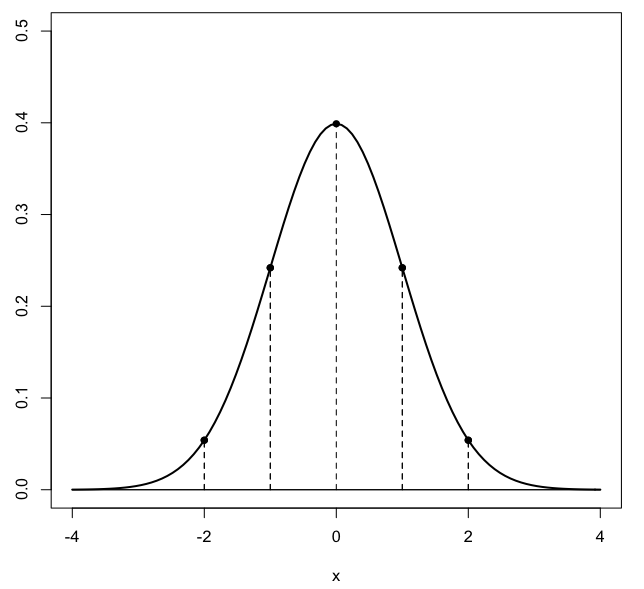
\includegraphics [scale=0.4] {gauss3.png} \end{center}

\title{Hanging chain}
\date{}

\begin{document}
\maketitle
\Large

The hanging chain, or catenary, is a famous problem solved by Johann Bernoulli about 1700.

\url{https://en.wikipedia.org/wiki/Johann_Bernoulli}

\begin{center} 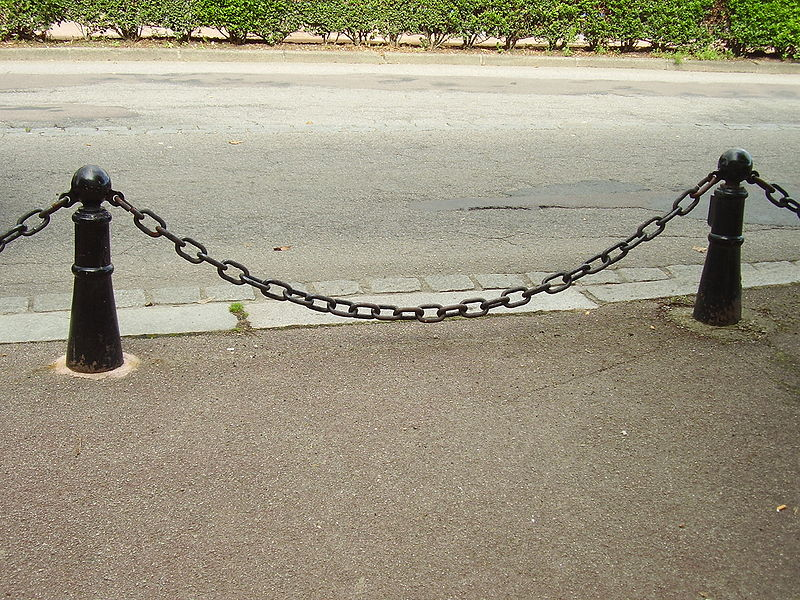
\includegraphics [scale=0.4] {hanging_chain2.jpg} \end{center}
   
\subsection*{solution}
This is quite a challenging problem.  See

\url{https://gordma.wordpress.com/2014/03/26/we-know-the-lion-by-his-claw/}

Bernoulli posed the problem as a public challenge, and said of Newton's anonymous submission:  "tanquam ex ungue leonem" ("we know the lion by his claw").

We imagine an ideal hanging cable (like the cable for a suspension bridge, without the vertical cables or bridge deck), although its ends might be at different heights.  The cable is ideal:  it will not stretch or contract, is perfectly flexible, and has constant mass per unit length. 

\begin{center} 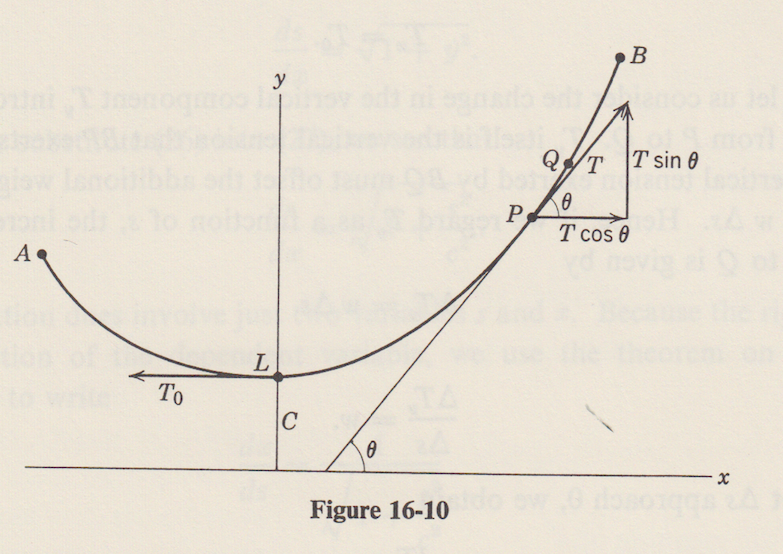
\includegraphics [scale=0.5] {Kline-16-10.png} \end{center}

Consider a position $P$ on the chain.  The part of the chain below $P$ pulls down on it, because of its weight, and the part above pulls up.  This force is called tension, $T$, and since the cable isn't moving, these forces are equal and opposite for every position on the chain.

The tension is in the direction of the angle $\theta$ tangent to the curve.  By convention it is positive upward.

We can decompose the tension $T$ into components in the $x$ and $y$ directions:

\[  T = T_x + T_y  \]
\[  T_x = T \cos \theta   \]
\[   T_y = T \sin \theta  \]
    
The curve traced out by the chain is described by $y = f(x)$, and it has a tangent at each point which is the ratio $T_y/T_x$.

\subsection*{moving to Q}

Now consider moving from $P$ up to the nearby point $Q$.  The weight acting at $Q$ is greater than that at $P$.  If the arc length of $L$ to $P$ is $s$, we add an additional small length $\Delta s$ to it in moving from $P$ to $Q$.  The weight of that little segment is the weight per unit length $w$, $\times \Delta s$.

The key point in the solution to this problem is that the additional force from the added weight changes $T_y$ (because gravity points downward), but does not affect $T_x$.  $T_x$ is the same at every point in the chain, including at the lowest point, which has no weight acting on it.  At this point, $L$, the tension is labeled as $T_0$, but $T_x$ is equal everywhere.

\[ T_x = T_0 \]

The change in $T_y$ when moving from $P$ to $Q$ is:
\[  \Delta T_y = w \Delta s \]
    
So
\[ \frac{\Delta T_y}{\Delta s} = w \]

and as we pass to the limit: 
\[ \frac{d T_y}{ds} = w \]

Since $w$ is a constant, this means that
\[ T_y = ws + D \]

where $D$ is a constant of integration.  But at $L$, both $s = 0$ and $T_y = 0$, so $D = 0$, and so:

\[ T_y = ws \]

This difference in $T_y$ at each point is what is responsible for the change in $\theta$ as we trace out the curve of the cable or chain.

\subsection*{Tangent}

From above:
\[ \frac{T_y}{T_x} = \frac{ws}{T_0} \]
    
but 
\[  \frac{T_y}{T_x} = \frac{T \sin \theta}{T \cos \theta} \]
so
\[  \frac{ws}{T_0} = \tan \theta \]

And $\tan \theta$ is the slope of the curve so
\[ y' = \tan \theta \]

Let $c = T_0/w$ so

\[  y' = \frac{ws}{T_0} = \frac{s}{c}  \]

\subsection*{Getting to x}

The second point of real insight required for this problem is that we now have a differential equation relating $y'$ to $s$, but we would like to have $y$ (and $y'$) as a function of $x$.

So finally, we need to relate $s$ to $x$ and $y$.  Recall that $s$ is arc length.  We know a formula for that:
\[ ds^2 = dx^2 + dy^2 \]

and
\[  \frac{ds}{dx} = \sqrt{1 + y'\ ^2} \]
\[ = \sqrt{1 + s^2/c^2} \]

Hence
\[  dx = \frac{1}{\sqrt{1 + s^2/c^2}} \ ds  \]
and our integral is
\[ \int \frac{s}{c}  \frac{1}{\sqrt{1 + s^2/c^2}} \ ds  \]

\subsection*{Integration}

We do two substitutions.  First, let $u = s/c$ and then $c \ du = ds$ so

\[  dx = c \frac{1}{\sqrt{1 + u^2}} \ du  \]

Second, because we have $\sqrt{1 + u^2}$, do a trig substitution with $u/1 = \tan t$.  Then $1/\sqrt{1 + u^2} = \cos t$, $\sqrt{1 + u^2} = \sec t$ and $du = \sec^2 t \ dt$ so

\[  \int dx = c \int \cos t \ \sec^2 t \ dt  \]
\[ = c \int \sec t \ dt \]

Integrate:

\[ x = c \ln | \sec t + \tan t |  \]
\[ = c \ln | \sqrt{1 + u^2} + u | \]
\[ = c \ln | \frac{s}{c} + \sqrt{1 + s^2/c^2} | \]

\subsection*{Solve for s}

Exponentiate:

\[  e^{x/c} = \frac{s}{c} + \sqrt{1 + s^2/c^2} \]

Let $z = s/c$.  Then
\[ (e^{x/c} - z)^2 = 1 + z^2 \]
\[ e^{2x/c} - 2 z e^{x/c} + z^2 = 1 + z^2 \]
\[ e^{2x/c} - 2 z e^{x/c} = 1 \]
\[ e^{x/c}(e^{x/c} - 2z) = 1 \]
\[ e^{x/c} - 2z = e^{-x/c} \]
\[ z = \frac{1}{2} (e^{x/c} - e^{-x/c}) \]
\[ s = c \ \frac{e^{x/c} - e^{-x/c}}{2} \]

\subsection*{Back to y}
Finally, recall that
\[  y' = \frac{s}{c} \]
    
So 
\[  y' = \frac{e^{x/c} - e^{-x/c}}{2} \]

Integrate:
\[ y = \frac{1}{2} \ c (e^{x/c} + e^{-x/c}) \]

This is the hyperbolic cosine.
\[ y = c \ \cosh \frac{x}{c} \]
    
And
\[ s = c \ \sinh \frac{x}{c} \]

Recall that $c = T_0/w$.  There is more to the problem (see Kline, for example), we need to figure out how $T_0$ depends on the geometry of the problem.  But, this seems a good place to stop.

Let's just plot it:

\begin{center} 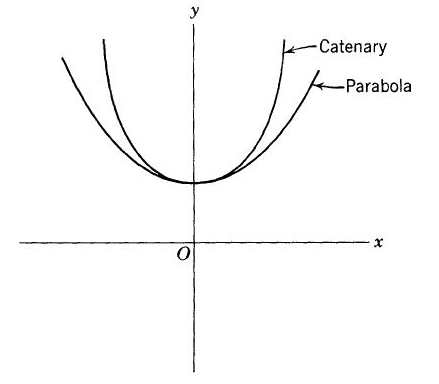
\includegraphics [scale=0.6] {catenary_parabola.png} \end{center}
It looks like a parabola but it's steeper.

\end{document}